\documentclass{article}
\usepackage{graphicx} % Required for inserting images

\title{Is Florida Getting Warmer?}
\author{An Dao}
\date{October 2025}

\begin{document}

\maketitle

\section{Results}
Having imported the Key West Annual Mean Temperature data (the basis for our Florida data), there was a correlation of:

\[ 0.5331784 \]

Out of one million random samples of temperatures and years, taken from the Florida data, not a single sample had a correlation greater than the Florida correlation (Figure 1).

\begin{figure}[h]
\begin{center}
    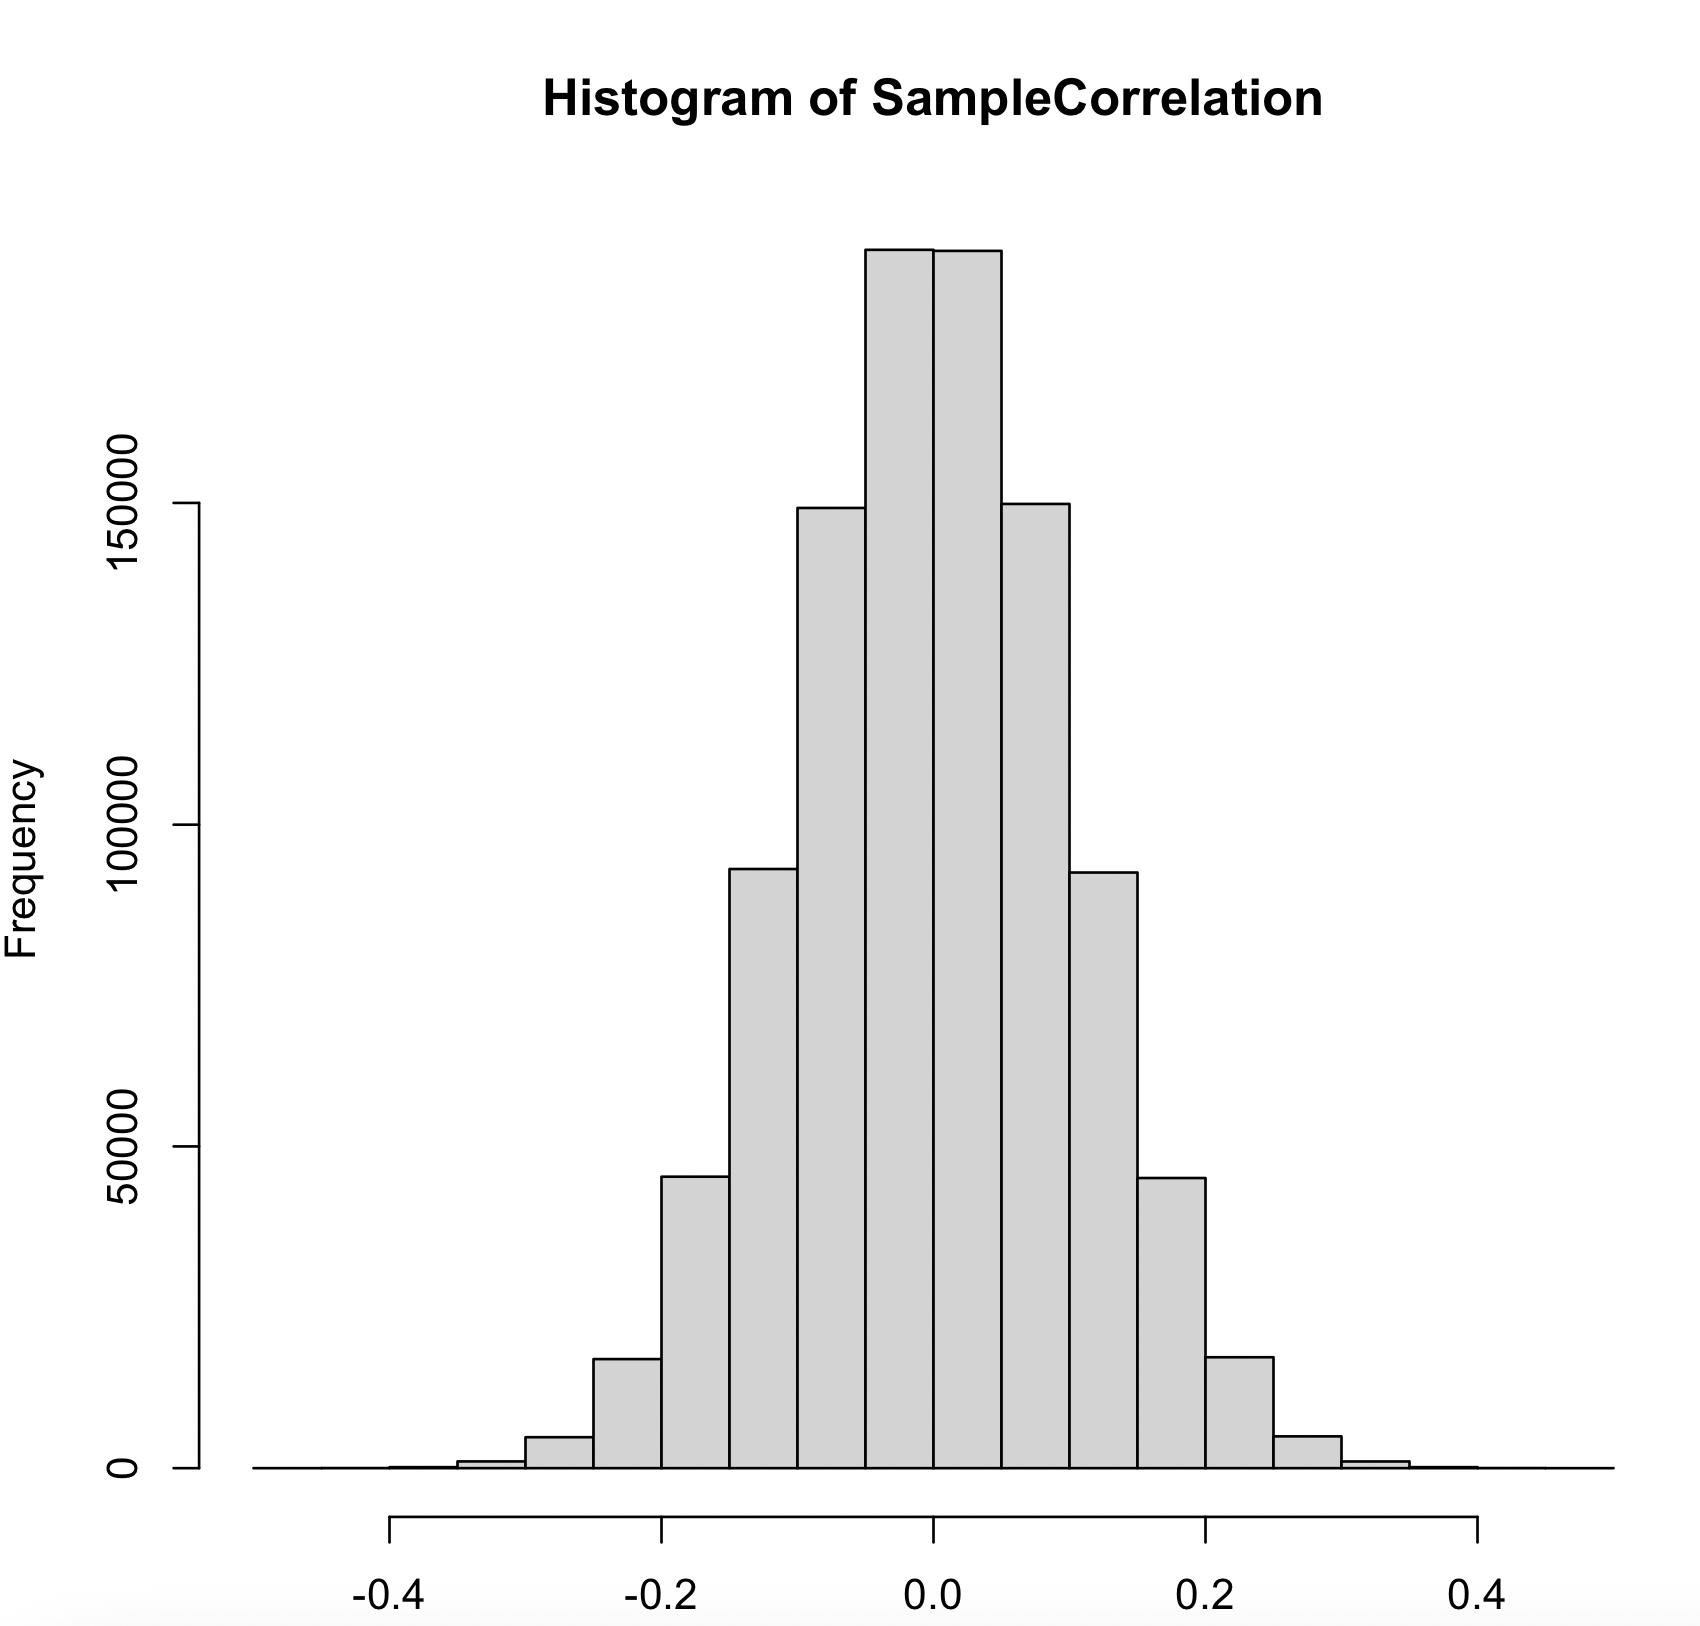
\includegraphics[width=.5\textwidth]{images/Histogram.png}\hfill
\end{center}
    \caption{Histogram of sampled correlations. Florida correlation is 0.53.}
\end{figure}

\section{Interpretation}
The Florida data is statistically significant as the rudimentary p-value is lower than 0.05. Any null hypothesis (there is no correlation between temperature and years in the Florida data) can be rejected.

\end{document}
